% -*- root: ../main.tex -*-
\subsection{Quadrocopterdynamik}
In der Literatur gibt es verschiedene dynamische Modelle für Quadrocopter mit unterschiedlicher Komplexität. In diesem Projekt wurde das Modell von \cite{LQR2013} verwendet. 
\subsection{Herleitung}
Für die Herleitung des Modelles hat sich als passender physikalischer Ansatz die Newton'schen - Bewegungsgleichungen bewährt. \\\\

Dazu lässt sich der Multikopter in drei Körpergruppen ($B_0, B_1, B_2$) einteilen: Bezugssystem (Startpunkt), ``nicht rotierende Körper'' (Grundplatte, Arme, Controller, Batterie, etc) und ``rotierende Körper'' (Motor, Rotor, Rotorschraube). In der Abbildung \ref{fig:schubkraefte} lassen sich die Schubkräfte $F_1, ... F_4$, wirkend im jeweiligen rotierenden System $B_{M1}, ..., B_{M2}$, erkennen.
\begin{figure}[ht]
  \centering
  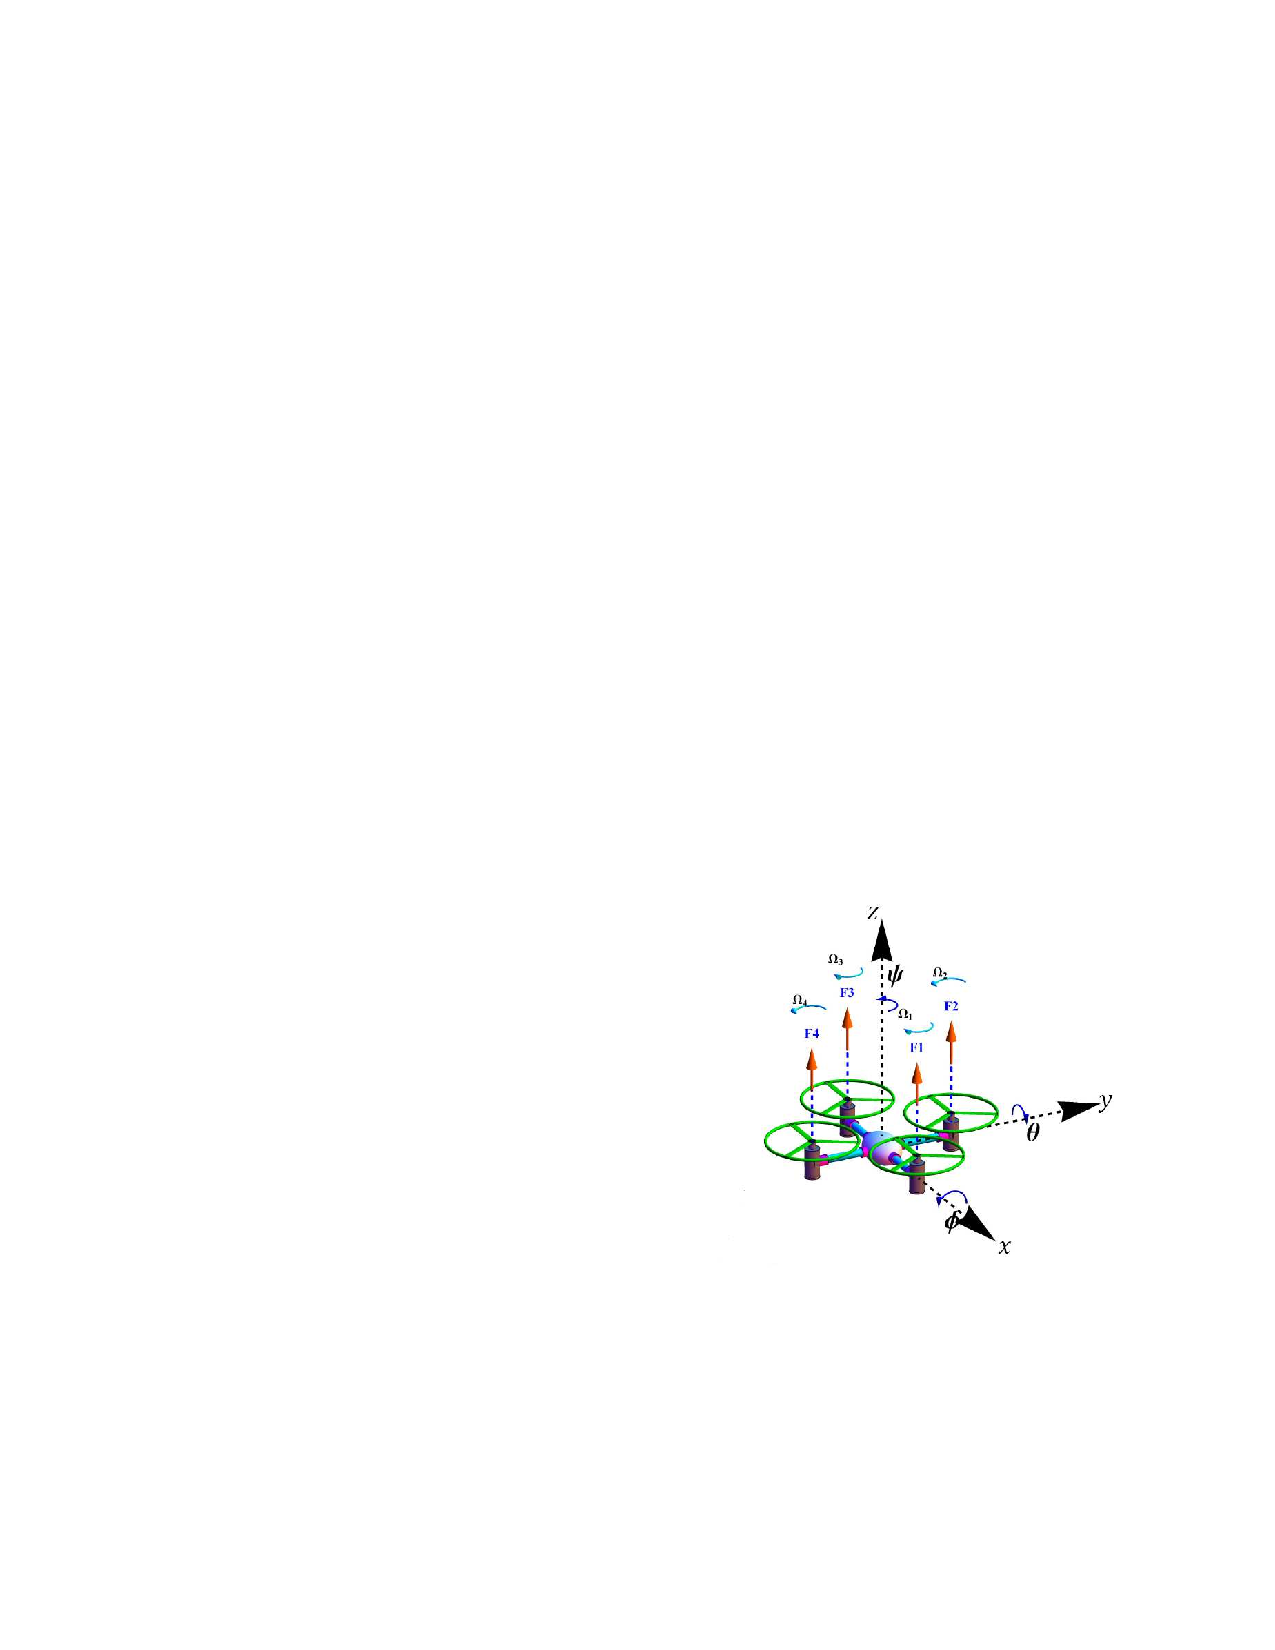
\includegraphics{images/MulticopterKraefte.pdf}
  \caption{Schubkräfte der Motoren}
  \label{fig:schubkraefte}
\end{figure} 

Im Folgendem entspricht \\
\begin{tabular}[t]{|l|l|}
  \hline
  $m_{ges}$ & Gesamtmasse des Multikopters \\ 
  $g$     & Gewichtskraft \\
  $I_{ges}$ & Gesamter Trägheitsmoment des Quadrocopters im System $B_1$\\
  ${_{M_i} I_{M_i}}$ & Trägheitmoment der Motoren im $i$-ten Motorsystem\\
  ${_{1}v_{1}}$ & Translatorische Geschwindigkeit des Körpers $B_1$ relativ zum $B_0$ System im $B_1$ System \\
  ${_{1}\omega_{1}}$ & Rotationsgeschwindigkeit des Körpers $B_1$ relativ zum $B_0$ System im $B_1$ System \\
  ${_{M_i} {\omega}_{1, M_i}}$ & Analog wie ${_{1}\omega_{1}}$\\
  ${_{M_i} {r}_{1, M_i}}$ & Abstand zwischen $B_{1}$ und $B_{2}$ mit Länge $d$ \\
  $A_{0,1}$ & Rotationsmatrix von Körper $B_1$ ins $B_0$ System \\
  $A_{1,M_i}$ & Rotationsmatrix von Körper $B_i$ ins $B_1$ System\\
  \hline
\end{tabular}\\

Mit der nicht eingezeichneten Gewichtskraft führt dies zu folgendem Kräftegleichgewicht im KOS($B_0$).
\begin{align}
    \frac{d}{dt} F_{ges} &= m_{ges} \cdot \frac{d}{dt} {_{1}v_{1}} = m_{ges} \frac{d_1}{dt} {_{1}v_{1}} + {_{1}\omega_{1}} \times m_{ges} {_{1}v_{1}} \\
    &=  {_{1}F_g} + \sum_{i = 1}^{4}{_{1}F_{i}}  \\\notag
    &= m_{ges} A_{1, 0} \cdot \begin{pmatrix} 0 \\ 0 \\ -g \end{pmatrix} + \sum_{i = 1}^4 {A_{1, M_i} \cdot _{M_i}F_{M_i}} \\
    &= m_{ges} A_{1, 0} \cdot \begin{pmatrix} 0 \\ 0 \\ -g \end{pmatrix} + \sum_{i = 1}^4 {\begin{pmatrix} 0 \\ 0 \\ F_i \end{pmatrix}}
\end{align}

Die Rotationsmatrix $A_{1, M_i}$ ändert sich je nach Konfiguration des Multikopters. Die Abbildung \ref{fig:Konfigurationen} zeigt die behandelten Konfigurationen.
\begin{figure}[ht]
  \centering
  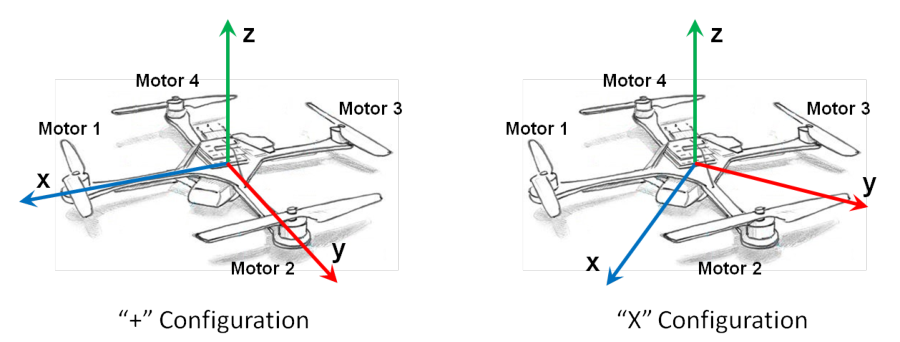
\includegraphics{images/Konfigurationen.pdf}
  \caption{Konfigurationen}
  \label{fig:Konfigurationen}
\end{figure}
Je nach Konfiguration entstehen folgende Konfigurationsmatrizen:\\\\
Für die ``+'' - Konfiguration werden folgende Matrizen verwendet:
\[
  A_{1, M_1} = \begin{pmatrix} 1 & 0 & 0 \\ 0 & 1 & 0 \\ 0 & 0 & 1 \end{pmatrix}
  A_{1, M_2} = \begin{pmatrix} 0 & -1 & 0 \\ 1 & 0 & 0 \\ 0 & 0 & 1 \end{pmatrix}
  A_{1, M_3} = \begin{pmatrix} -1 & 0 & 0 \\ 0 & -1 & 0 \\ 0 & 0 & 1 \end{pmatrix} 
  A_{1, M_4} = \begin{pmatrix} 0 & 1 & 0 \\ -1 & 0 & 0 \\ 0 & 0 & 1 \end{pmatrix}
\] \label{sec:konfg_matrix}
Für die ``x'' - Konfiguration werden folgende Matrizen verwendet:
\[
  A_{1, M_1} = \begin{pmatrix} \frac{\sqrt{2}}{2} & \frac{\sqrt{2}}{2} & 0 \\ \frac{-\sqrt{2}}{2} & \frac{\sqrt{2}}{2} & 0 \\ 0 & 0 & 1 \end{pmatrix} \hspace{0.5em}
  A_{1, M_2} = \begin{pmatrix} \frac{\sqrt{2}}{2} & -\frac{\sqrt{2}}{2} & 0 \\ \frac{\sqrt{2}}{2} & \frac{\sqrt{2}}{2} & 0 \\ 0 & 0 & 1 \end{pmatrix}
\]
\[
  A_{1, M_3} = \begin{pmatrix} -\frac{\sqrt{2}}{2} & -\frac{\sqrt{2}}{2} & 0 \\ \frac{\sqrt{2}}{2} & -\frac{\sqrt{2}}{2} & 0 \\ 0 & 0 & 1 \end{pmatrix} \hspace{0.5em}
  A_{1, M_4} = \begin{pmatrix} -\frac{\sqrt{2}}{2} & \frac{\sqrt{2}}{2} & 0 \\ -\frac{\sqrt{2}}{2} & -\frac{\sqrt{2}}{2} & 0 \\ 0 & 0 & 1 \end{pmatrix}
\]
\\
Für das Kräftegleichgewicht sind die Matrizen nicht relevant, jedoch für den folgenden Drallsatz im körperfesten System $B_1$. %Zuvor wird der Drallsatz im körperfesten System der Motoren betrachtet. Dort wirkt dem Drehmoment der Motoren $M_i$ ein Reaktionsdrehmoment  $\tau_i$ entgegen:
Zuvor wird ein fest montierter Motor betrachtet mit dem Drehmoment $M$. Diesem wirkt ein Strömungswiderstand $\tau_{drag}$ entgegen und es gilt: 
\begin{align}
{I_{rot}} \cdot \dot{\omega}  = M - \tau_{drag} 
\end{align}

Dabei ist $I_{rot}$ das Trägheitsmoment des Rotors entlang seiner z-Achse. Der Strömungswiderstand ist in der Literatur \cite{LQR2013} folgenderweise definiert als:
\begin{align}
    \tau_{drag} = \frac{1}{2} \rho A_r v^2
\end{align}
$\rho$ ist die Luftdichte, $A_r$ die Fläche, die der Rotor bei der Umdrehung überschreitet und $v$ ist die Geschwindigkeit relativ zur Luft. Näherungsweise gilt: $\omega \approx \frac{v}{r}$ und es folgt:
\begin{align}
    \tau_{drag} \approx k_{drag} \omega^2
\end{align}
Die Konstante $k_{drag} > 0$ ist abhängig von der Luftdichte, dem Radius, der Form des Propellers und anderen Faktoren. Für quasistationär Manöver ist $\omega$ konstant und es gilt: 
\begin{align}\label{gl:MDrag}
    M = \tau_{drag} \approx k_{drag} \omega^2 
\end{align}

Neben dem Drehmoment der Rotoren wird auch deren Schubkraft benötigt. Die Literatur \cite{LQR2013} gibt folgende Formel an:
\begin{align}
    F_s = C_T \rho A_r r^2 \omega^2 
\end{align}
$C_T$ ist der Schubkoeffizient für einen speziellen Rotor, $\rho, A_r$ ist wie oben, die Dichte der Luft bzw. die Fläche die, der Rotor bei der Umdrehung überschreitet. Analog führen wir einen vereinfachten Koeffizienten ein:

\begin{align}\label{gl:schub}
    F_s \approx k_{T} \omega^2 
\end{align}

Im Folgenden wird die Annahme getroffen, dass sich der Quadrocopter in einem quasistationären Zustand befindet, d.h. $\omega = const$\\

Dann gilt für Drallsatz im $B_{M_i}$ System: 
\begin{align}
    {_{M_i} I_{M_i}} {_{M_i} \dot{\omega}_{M_i}} &+ {_{M_i} {\omega}_{1}} \times {_{M_i} I_{M_i}} {_{M_i} {\omega}_{M_i}} = {_{M_i} I_{M_i}} \left({_{M_i} \dot{\omega}_{1}} + {_{M_i} \dot{\omega}_{1, M_i}}\right) \\
    &+ {_{M_i} {\omega}_{1}} \times {_{M_i} I_{M_i}} \left({_{M_i} {\omega}_{1}} + {_{M_i} {\omega}_{1, M_i}} \right) \underbrace{\approx}_{{_{M_i} {\omega}_{1}} << {_{M_i} {\omega}_{1, M_i}}} {_{M_i} I_{M_i}} {_{M_i} \dot{\omega}_{1,M_i}} \\
    &+ {_{M_i} {\omega}_{1}} \times {_{M_i} I_{M_i}} {_{M_i} {\omega}_{1, M_i}} = M_i - {_{M_i} \tau_{M_i}}
\end{align}
Zudem folgt wegen Stationärflug:
\begin{align}
    \underbrace{{_{M_i} I_{M_i}} {_{M_i} \dot{\omega}_{1, M_i}}}_{=0\text{, da }\omega =\text{ const}} + {_{M_i} {\omega}_{1}} \times {_{M_i} I_{M_i}} {_{M_i} {\omega}_{1, M_i}} = {_{M_i} {\omega}_{1}} \times {_{M_i} I_{M_i}} {_{M_i} {\omega}_{1, M_i}} =  M_i - {_{M_i} \tau_{M_i}} 
\end{align}
Dem Drehmoment der Motoren $M_i$ wird ein Gegendrehmoment ${_{M_i}\tau_{M_i}}$ entgegen gesetzt. Dieses Drehmoment findet sich auch wieder im Drallsatz des System $B_{1}$

\begin{align}
    I_{ges} {_{1} \dot{\omega}_{1}} + {_{1} {\omega}_{1}} \times I_{ges} {_{1} {\omega}_{1}} = (\tau_{R} + \tau_{P}) -\sum_{i = 1}^{4} {_{1} \tau_{M_i}} 
\end{align}

Die Drehmomente $\tau_R$ und $\tau_P$ ergeben sich aus den Roll $f_2 + f_4$ - und Nickkräfte $f_1 + f_3$: 
\begin{align}
    \tau_R = A_{1, M_1} {_{M_1}r_{1, M_1}} \times F_1  +  A_{1, M_3} {_{M_3}r_{1, M_3}} \times F_3 \\
    \tau_P = A_{1, M_2} {_{M_2}r_{1, M_2}} \times F_2  +  A_{1, M_4} {_{M_4}r_{1, M_4}} \times F_4
\end{align}

Das Gegendrehmoment ${_{M_i} \tau_{M_i}}$ ist äquivalent mit ${_{1} \tau_{M_i}}$, da der Übergang von System $B_{M_i}$ ins $B_{1}$ System eine Rotation um die z-Achse darstellt und ${{M_i} \tau_{M_i}}$ nur eine z-Komponente besitzt. Somit folgt für den ganzen Drallsatz:

\begin{align}
    I_{ges} {_{1} \dot{\omega}_{1}} + {_{1} {\omega}_{1}} \times I_{ges} {_{1} {\omega}_{1}} &+ \sum_{i=1}^{4}{{_{1} {\omega}_{1}} \times {_{M_i} I_{M_i}} {_{M_i} {\omega}_{1, M_i}}} \\
    &= -\sum_{i = 1}^{4}{M_i} + (\tau_{R} + \tau_{P})
\end{align}
$I_{ges}$ stellt das Trägheitsmoment des Körpers 1, d.h. des Quadrokopters ohne rotierende Objekte, dar. ${_{M_i} I_{M_i}}$ hingegen ist das Trägheitsmoment, eines einzelnen Rotors $i$. Bei Brushlesh Motoren ist es so, das sich die ``Wand'' mitdreht. Dies muss die Kalkulation des Trägheitsmomentes ${_{M_i} I_{M_i}}$ mit einbezogen werden.\\
Da ${_{M_i} {\omega}_{1, M_i}}$ nur eine z - Komponente besitzt mit $\omega_{M_i}$, lässt sich Gleichung folgendermassen vereinfachen.
\begin{align}
    I_{ges} {_{1} \dot{\omega}_{1}} + {_{1} {\omega}_{1}} \times I_{ges} {_{1} {\omega}_{1}} &+ \sum_{i=1}^{4}{({_{1}{\omega}_{1}} \times e_z) \cdot I_{M} \omega_{M_i} } \\
    &= \begin{bmatrix} 0 \\ 0 \\ -\sum_{i = 1}^{4}{M_i} \end{bmatrix} + (\tau_{R} + \tau_{P})
\end{align}\\\\
Für die + Konfiguration entsteht mit \ref{sec:konfg_matrix} nun folgendes Modell:
\begin{align}
    {_{0}\dot{r}_{1}} &= A_{0, 1} {_{1}v_{1}} \\
    m_{ges} \frac{d_1}{dt} {_{1}v_{1}} &+ {_{1}\omega_{1}} \times m_{ges} {_{1}v_{1}} = m_{ges} A_{1, 0} \cdot \begin{pmatrix} 0 \\ 0 \\ -g \end{pmatrix} + \sum_{i = 1}^4 {\begin{pmatrix} 0 \\ 0 \\ F_i \end{pmatrix}} \\
    {{\dot{A}_{0, 1}}} &= {A_{0, 1}} \tilde{_{1} {\omega}_{1}}\\
    I_{ges} {_{1} \dot{\omega}_{1}} &+ {_{1} {\omega}_{1}} \times I_{ges} {_{1} {\omega}_{1}} + \sum_{i=1}^{4}{({_{1}{\omega}_{1}} \times e_z) \cdot I_{M} {_{M_i}\omega_{M_i}} } \\
    &= \begin{bmatrix} 0 \\ 0 \\ -\sum_{i = 1}^{4}{M_i} \end{bmatrix} + (\tau_{R} + \tau_{P}) = \begin{bmatrix} d(F_2 - F_4) \\ d(F_3 - F_1) \\ -\sum_{i = 1}^{4}{M_i} \end{bmatrix}
\end{align}

Mit \ref{gl:MDrag} und \ref{gl:schub}
\begin{align}
    {_{0}\dot{r}_{1}} &= A_{0, 1} {_{1}v_{1}} \\
    m_{ges} \frac{d_1}{dt} {_{1}v_{1}} &+ {_{1}\omega_{1}} \times m_{ges} {_{1}v_{1}} = m_{ges} A_{1, 0} \cdot \begin{pmatrix} 0 \\ 0 \\ -g \end{pmatrix} + {\begin{pmatrix} 0 \\ 0 \\ \sum_{i = 1}^4 k_{T} {_{M_i}\omega^2_{1, M_i}} \end{pmatrix}} \\
    {{\dot{A}_{0, 1}}} &= {A_{0, 1}} \tilde{_{1} {\omega}_{1}}\\
    I_{ges} {_{1} \dot{\omega}_{1}} &+ {_{1} {\omega}_{1}} \times I_{ges} {_{1} {\omega}_{1}} + \sum_{i=1}^{4}{({_{1}{\omega}_{1}} \times e_z) \cdot I_{M} {_{M_i}\omega_{M_i}} } \\
    &= \begin{bmatrix} 0              & d \cdot k_{T} & 0             & -d \cdot k_{T} \\ 
                       -d \cdot k_{T} & 0             & d \cdot k_{T} & 0  \\
                       -k_{drag}      & k_{drag}      & -k_{drag}    & k_{drag}
       \end{bmatrix}
    \cdot 
    \begin{bmatrix}
      {_{M_1} {\omega}^2_{M_1}} \\
      {_{M_2} {\omega}^2_{M_2}}\\
      {_{M_3} {\omega}^2_{M_3}}\\
      {_{M_4} {\omega}^2_{M_4}}
    \end{bmatrix}
\end{align}
\subsubsection{Quaternionen}\label{subsub:Quaternionen}
Statt mit Eulerwinkel wird die Rotationsmatrix $A_{0, 1}$, welche die Vektoren vom Bezugssystem ins Körpersystem transformiert, mit Hilfe von Quaternionen berechnet. Dies bringt den Vorteil das kritische Punkte, also Punkte dessen Zuordnung nicht lokal umkehrbar, nicht spezifisch betrachtet werden müssen. Es bringt aber den Nachteil mit sich, dass für eine sinnvolle Auswertung der Quaternionen, diese normiert sein müssen.
\\
Die Rotationsmatrix für Quaternionen lautet: 
\begin{align}
A_{0, 1} := R_{0, 1}(q) = \left[ \begin{matrix} 1-2(q_2^2 + q_3^2) &
-2q_0q_3+2q_1q_2 &
2q_0q_2+2q_1q_3 \\
2q_0q_3+2q_1q_2 &
1-2(q_1^2 + q_3^2) &
-2q_0q_1+2q_2q_3 \\
-2q_0q_2+2q_1q_3 &
2q_0q_1+2q_2q_3 &
1-2(q_1^2 + q_2^2)
\end{matrix}
\right]
\end{align}
nach \cite{Richter2009}.\\ 
Die Zeitableitung der Quaternionen $q$ lässt nach \cite{Chou1992}, wie folgt berechnen: $\dot q = \frac{1}{2} q \otimes \begin{bmatrix} 0 \\ \omega \end{bmatrix}$. \\
\\
Somit folgt für das dynamische System des Quadrocoptors in der ``+''- Konfiguration:
\begin{align}
    {_{0}\dot{r}_{1}} &= R_{0, 1}(q) {_{1}v_{1}} \\
    \dot q &= \frac{1}{2} q \otimes \begin{bmatrix} 0 \\ \omega \end{bmatrix} \\
    m_{ges} \frac{d_1}{dt} {_{1}v_{1}} &+ {_{1}\omega_{1}} \times m_{ges} {_{1}v_{1}} = R(q)^T \begin{pmatrix} 0 \\ 0 \\ -m_{ges} \cdot g \end{pmatrix} + {\begin{pmatrix} 0 \\ 0 \\ \sum_{i = 1}^4 k_{T} {_{M_i}\omega^2_{1, M_i}} \end{pmatrix}} \\
    I_{ges} {_{1} \dot{\omega}_{1}} &+ {_{1} {\omega}_{1}} \times I_{ges} {_{1} {\omega}_{1}} + \sum_{i=1}^{4}{({_{1}{\omega}_{1}} \times e_z) \cdot I_{M} {_{M_i}\omega_{M_i}} } \\
    &= \begin{bmatrix} 0              & d \cdot k_{T} & 0             & -d \cdot k_{T} \\ 
                       -d \cdot k_{T} & 0             & d \cdot k_{T} & 0  \\
                       -k_{drag}      & k_{drag}      & -k_{drag}    & k_{drag}
       \end{bmatrix}
    \cdot 
    \begin{bmatrix}
      {_{M_1} {\omega}^2_{M_1}} \\
      {_{M_2} {\omega}^2_{M_2}}\\
      {_{M_3} {\omega}^2_{M_3}}\\
      {_{M_4} {\omega}^2_{M_4}}
    \end{bmatrix}
\end{align}

Da die Schrittweite des ODE - Lösers in unserem Lösungsansatz deutlich kleiner als 1 ist, wird die Normierung der Quaternionen mit Hilfe des Korrekturterms 
\begin{align}
  \begin{matrix}
    q_1 = ... + \lambda \dot q_1\\
    q_2 = ... + \lambda \dot q_2\\
    q_3 = ... + \lambda \dot q_3\\
    q_4 = ... + \lambda \dot q_4\\
    \text{mit } \lambda = 1- (q_1^2 + q_2^2 + q_3^2 +q_4^2)
  \end{matrix}
\end{align} gelöst \cite{Cooke1992}.

Für das Projekt wurde nun $\dot{x} = f(x, u) \in \R^{13}$ wie folgt gewählt:
\begin{align}\label{gl:ODE}
  f(x, u) &:= 
  \begin{bmatrix}
    R_{0, 1}(q) {_{1}v_{1}} \\
    \frac{1}{2} q \otimes \begin{bmatrix} 0 \\ \omega \end{bmatrix} \\
    M^{-1} (T - \Theta)
  \end{bmatrix} \\
  \text{mit } 
  T &:= \begin{bmatrix} 0\\ 0\\ -k_T \cdot \sum_{i=0}^{4}  {_{M_i} {\omega}^2_{M_i}}^2 \\ 
   K \cdot \begin{bmatrix} {_{M_1} {\omega}^2_{M_1}}^2 \\ {_{M_2} {\omega}^2_{M_2}} \\ {_{M_3} {\omega}^2_{M_3}} \\ {_{M_4} {\omega}^2_{M_4}} \end{bmatrix} +  \begin{bmatrix} 0 \\ 0 \\ 1\end{bmatrix} \times {_{1}\omega_{1}} \cdot I_M \cdot ({_{M_1} {\omega}^2_{M_1}} - {_{M_2} {\omega}^2_{M_2}} + {_{M_3} {\omega}^2_{M_3}} - {_{M_4} {\omega}^2_{M_4}})
  \end{bmatrix}
  \text{, } \\
  \Theta &:= \begin{bmatrix} m_{ges} \cdot {_{1}\omega_{1}} \times {_{1}v_{1}} + R(q)^T \cdot \begin{bmatrix} 0 \\ 0 \\ g \end{bmatrix} 
  \end{bmatrix} \text{ und } \\
  M &:= diag(m, m, m, I_{ges_1}, I_{ges_2}, I_{ges_3}) \text{ sowie für }\\
  x &:=[r_1, r_2, r_3, q_1, q_2, q_3, q_4, v_1, v_2, v_3, \omega_1, \omega_2, \omega_3 ] \text{ und } \\
  u &:=[{_{M_1} {\omega}_{M_1}}, {_{M_2} {\omega}_{M_2}}, {_{M_3} {\omega}_{M_3}}, {_{M_4} {\omega}_{M_4}}]\\
  K&:= \begin{bmatrix} 0              & d \cdot k_{T} & 0             & -d \cdot k_{T} \\ 
                       -d \cdot k_{T} & 0             & d \cdot k_{T} & 0  \\
                       -k_{drag}      & k_{drag}      & -k_{drag}    & k_{drag}
       \end{bmatrix}
\end{align}





